\section{Ordine del giorno}
\begin{enumerate}
\item Discussione sulle tecnologie 
\item Pianificazione per prima revisione
\item Metodo Agile
\item Coordinamento interno 
\end{enumerate}

\subsection{Discussione sulle tecnologie}
\subsubsection{Librerie Standard OpenIDVC/VP}
Dopo il lavoro di ricerca interno effettuato si sono prodotti alcuni documenti tecnici che il team ha provveduto a leggere.\\
Due tra i più importanti sono stati architetturaEUDI.pdf e ricercaOpenID.pdf.\\
Dalle precendenti discussioni fatte, dai meeting fatti con l'azienda e da una analisi dei documenti precendenti siamo giunti alla 
conclusione che per utilizzare lo standard OpenIDVC/VP dobbiamo uttilizzare una libreria preesistente.\\
Nonostante la documentazione dello standard sia abbondante preferiamo non implementare lo standard con una libreria scritta da noi.\\
I vantaggi di utilizzare una libreria esistente sono l'avere la sicurezza di rispettare a pieno lo standard e il velocizzare questo dettaglio implementativo che altrimenti ci richiederebbe una quantità di tempo maggiore.\\
Come documentato nel documento ricercaOpenID.pdf nel capitolo 4, tra le librerie che abbiamo trovato quella che ci ha colpito maggiormente è
Waltid ssikit, si rimanda al spotraindicato documento per riferimenti e dettagli.\\
Il motivo maggiore che ci ha fatto scegliere questa libreria è una buona documentazione offerta, e la possibilità di fare il deploy di un container docker in grado successivamente di
gestire in autonomia le richieste che gli si fanno.\\
Abbiamo evidenziato che tra le varie metodologie proposte per utilizzare la libreria quella che utilizzeremo sarà la REST API.
Con questa libreria riusciamo ad implementare il Wallet, la parte del Issuer e la parte del Verifier.\\
Utilizzando questa libreria tuttavia ci vengono dei dubbi legati al fatto che attraverso un unico Server all'interno di un unico container docker si riescono a fornire tutte le 
interfacce legate alle certificazioni per tutti e 3 gli attori del progetto, quindi il dubbio che ci viene è se conviene fare il deploy di questo
SSID KIT 3 volte, oppure possiamo mantenerne solo uno, tuttavia rinunciando al concetto di decentralizzazione evidenziato nella ricerca
della architetturaEUDI.pdf.\\
Un'altro dubbio che ci viene è che questa libreria sia ad un livello troppo alto, e ai fini didattici e del progetto non ci convenga magari 
utilizzare uno strumento più a livello basso, che ci avvicini maggiormente allo standard e che tuttavia non ci offra uno strumento ready-to-use come WaltID.\\
Al di là di che libreria utilizzeremo per gestire le credenziali e la comunicazione per le credenziali, siamo abbastanza sicuri che la
utilizzeremo attraverso una comunicazione REST API.\\
Quest'ultimo dettaglio implementativo è dato dalla natura del progetto che ci richiede la creazione di webapp.\\
Nel caso fosse stato necessario realizzare
una app mobile ci sarebbero state altre soluzioni possibilmente realizzabili, come librerie implementabili per linguaggi di programmazione come Kotlin, implementabili tramite Maven/Grandle.\\

\subsubsection{Struttura architetturale componenti}
Abbiamo analizzato e documentato tramite analisi del capitolato, ricerca dei requisiti e altri documenti tecnici la struttura che i componenti architetturali finali dovranno avere.\\
Ai fini del prodotto finito e anche per la PoC (Proof Of Concept) il lavoro sarà consegnato tramite container docker pronto per fare il deploy.\\
Utilizzando lo strumento di container di docker si utilizzerà una virtualizzazione che ci permetterà di essere indipendenti dal sistema operativo utilizzato, ci garantirà maggiore compatibilità tra i componenti e ci fornirà una più semplice metodologia per fare il deploy del nostro prodotto.\\
Saranno realizzate le seguenti componenti, di seguito nel testo ci si riferirà a loro tramite l'acronimo iniziale nella seguente lista:
\begin{itemize}
	\item \textbf{BOC}: webapp back-office component
	\item \textbf{IUIC}: Issuer demo user interaction component 
	\item \textbf{VUIC}: Verifier demo user interaction component 
	\item \textbf{Wallet}: Wallet front-end webapp
\end{itemize}
Tutte le seguenti informazioni sono solo proposte ed osservazioni, le decisioni finali per il PoC e per il progetto dovranno ancora essere prese in base alle seguenti osservazioni e a successivi colloqui con la azienda.\\
\\
Tenendo in considerazione il documento analisiDeiRequisiti.pdf, capitolo 3.4, come evidenziato dagli Use Case UC01/2/3 la realizzazione
del component BOC e IUIC dovranno avere un database accessibile in comune.\\
Un utente potrà richiedere una credenziale nella IUIC, la sua richiesta verrà memorizzata all'interno di un database, un officer accederà
dalla BOC allo stesso database per effettuare l'approvazione del rilascio della credenziale, la suddetta credenziale verrà memorizzata all'interno del database.\\
In fine l'utente andrà nella IUIC per ottenere la sua credenziale.\\
Per realizzare la BOC e la IUIC si è pensata ad due webapp distinte ed un database in comune.\\
Questa decisione rispecchia anche un utilizzo reale dato che un eventuale Issuer (es. UNIPD) sarà il responsabile
per entrambe le piattaforme e sarà responsabile anche per il database utilizzato da entrambe.\\
\\
Per la realizzazione del VUIC si è pensato alla realizzazione di una semplice webapp, dato che questo componenente è semplicemente una demo una volta presentata una credenziale
non ci saranno funzioni e servizi che il Verifier potrà fornire, quindi è sufficiente una webapp che riceverà la credenziale di presentazione fornita e darà un messaggio di successo nella operazione.
\\
Per la realizzazione del Wallet sarà necessario una webapp.\\
Per garantire gli Use Case UC04/5 sarà necessario utillizzare un sistema per memorizzare le credenziali.\\
Bisogna capire se il wallet dovrà essere il cloud oppure in locale (stile metamask).\\
Come specificato da direttive nella archittetturaEUDI a noi ci sembra più naturale il realizzare una versione in locale del wallet.\\
Sarà hostata solo la webapp, non saranno presenti database su nessun server e tutte le credenziali saranno memorizzate all'interno del LocalStorage del Browser.\\

\subsubsection{Tecnologie Da Utilizzare}
Per la realizzazione delle webapp sopra citate si è fatta una ricerca su eventuali framework da utilizzare.\\
Due framework che abbiamo analizzato sono stati Svelte e React.\\
I punti a favore di Svelte sono:
\begin{itemize}
	\item Fine progetto compilato in un budle.js
	\item Il budle è molto leggero
	\item Non esiste una virtual DOM
\end{itemize}
I suddetti punti elencati sopra sono a sua volta anche punti a sfavore di questa libreria in quanto non si ha un compilazione in tempo reale,
ed il fatto che non esista un virtual DOM ci dà una difficoltà maggiore nel navigare la DOM classica di HTML.\\
In fine è stato evidenziato come questo framework sia utilizzabile più per progetti casalinghi e non per progetti grandi e con uno sviluppo ampio.\\
\\
I punti a favore di React sono:
\begin{itemize}
	\item Maggiore supporto, framework molto maturo
	\item Framework basato sui component
	\item Possibilità di utilizzare typescript
	\item Maggiore documentazione online
	\item Curva di apprendimento più blanda
\end{itemize}
Nonostante React abbia la possibilità di utilizzare typescript è stato evidenziato come questa possibilità sia negativa in quanto i benefici non superano gli aspetti negativi come il non trovare successivamente documentazione 
adatta online, oppure il seguire un linguaggio tipizzato per la realizzazione di webapp che tuttosommato non richiedono la implementazione di funzioni complicate o complesse.\\
\\
Esistono successivamente anche altri framework, che analizzeremo a breve.\\
Abbiamo escluso a priori Angular in quanto nonostante sia molto maturo e usato ampiamente in ambito business ha una curva di apprendimento molto lenta e 
date le basi da cui i membri del gruppo partono, non ci permetterebbe la buona riuscita del progetto.\\\\
Per quanto riguarda i database da realizzare bisogna fare una scelta implementativa molto importante legata al tipo di BDMS.\\
Una soluzione classica che tutti i membri del gruppo sarebbero in grado di fare sarebbe l'implementare un DBMS SQL come per esempio postgressSQL oppure MySQL.\\
Facendo questa scelta bisognerebbe creare anche un backend con cui reperire le informazioni dal DB e fornirle in forma di API al frontend.\\
Una possibilità sarebbe utilizzando il linguaggio di programmazione PHP, conosciuto da tutti i membri del gruppo e utilizzato già per 
precedenti progetti.\\
Questa soluzione sarebbe la più semplice dato che utilizzerebbe tecnologie già conosciute dal team, tuttavia sarebbe anche la più lunga dato che tra database e webapp
si dovrebbe implementare un backend, e questo richiederebbe tempi maggiori di programmazione per questa porzione.\\
\\
Una soluzione alternativa sarebbe utilizzare un DBMS NoSQL come per esempio Redis oppure MongoDB.\\
Queste soluzioni sono più compatibili con una moderna webapp, richiederebbe meno codice e si avrebbe una maggiore semplicità realizzativa.\\
Richiederebbe però studiare ed imparare nuove tecnologie come Redis oppure Node.js.\\

\subsection{Pianificazione per prima revisione}
Il team a fronte della prima revisione RTB ha stilato una lista delle cose da fare procedendo all'indietro.Creando una lista delle cose da fare inserite poi all'interno di una linea temporale con data ultima quella della prima revisione.
Questa linea temporale verrà poi approfondita nella sezione successiva "\textit{Metodo Agile}".


\subsection{Metodo Agile}
Dato lo svolgimento del progetto il gruppo ha deciso di adottare un metodo di lavoro agile al fine di aumentare la produttività.
Si è optato per un modello SCRUM e in vista della prima revisione si sono previsti 3 periodi di sprint ciascuno di 2 settimane. 
Per ogni sprint si è pianificato il lavoro da fare in modo tale da non doverlo organizzare nel periodo stesso dello svolgimento.
Di seguito la figura rappresentante la linea temporale in vista della prima revisione e i tre sprint nello specifico. 
\begin{center}
	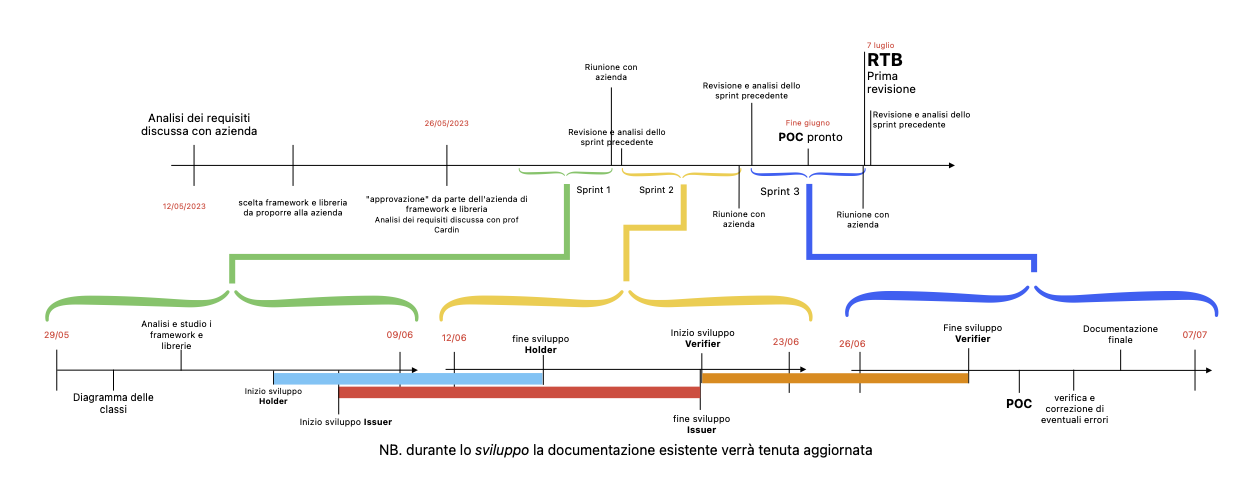
\includegraphics[scale = 0.35]{./res/images/RTB-1a-revisione.png}
\end{center}

\subsection{Coordinamento interno}
Si è fatto il punto della situazione sul lavoro effetuato durante la settimana corrente ed il gruppo si è sincronizzato e allineato; il responsabile inoltre ha suddiviso i ruoli e le mansioni da svolgere la settimana seguente. 
